\documentclass[11pt,a4paper]{article}

% ── Packages ──
\usepackage[margin=0.9in]{geometry}
\usepackage{graphicx}
\usepackage{booktabs}
\usepackage{amsmath,amssymb}
\usepackage{hyperref}
\usepackage{tikz}
\usetikzlibrary{shapes.geometric, arrows.meta, positioning, fit, backgrounds, calc}
\usepackage{listings}
\usepackage{xcolor}
\usepackage{caption}
\usepackage{subcaption}
\usepackage{enumitem}
\usepackage{float}
\usepackage{fancyhdr}
\usepackage{titlesec}
\usepackage{setspace}
\usepackage{tabularx}
\usepackage{multirow}
\usepackage{array}
\usepackage[T1]{fontenc}
\usepackage{lmodern}
\usepackage{microtype}
\usepackage[numbers]{natbib}

\hypersetup{
    colorlinks=true,
    linkcolor=blue!70!black,
    citecolor=green!50!black,
    urlcolor=blue!60!black
}

\pagestyle{fancy}
\fancyhf{}
\fancyhead[L]{\small CSE 4122 -- NLP Project Report}
\fancyhead[R]{\small Interpretable SE Sentiment Classification}
\fancyfoot[C]{\thepage}
\renewcommand{\headrulewidth}{0.4pt}

\singlespacing

\lstset{
    basicstyle=\ttfamily\small,
    backgroundcolor=\color{gray!8},
    frame=single,
    framerule=0.3pt,
    rulecolor=\color{gray!50},
    breaklines=true,
    columns=fullflexible,
    keepspaces=true
}

% ── TikZ Styles ──
\tikzstyle{stage} = [
    rectangle, rounded corners=4pt, minimum width=3.2cm, minimum height=0.9cm,
    text centered, draw=blue!60!black, fill=blue!8, font=\small\bfseries,
    line width=0.6pt
]
\tikzstyle{module} = [
    rectangle, rounded corners=3pt, minimum width=2.6cm, minimum height=0.7cm,
    text centered, draw=teal!70!black, fill=teal!6, font=\small,
    line width=0.5pt
]
\tikzstyle{data} = [
    cylinder, shape border rotate=90, draw=orange!70!black, fill=orange!6,
    minimum width=2cm, minimum height=0.7cm, font=\small,
    line width=0.5pt, aspect=0.25
]
\tikzstyle{arrow} = [-{Stealth[length=5pt]}, thick, color=blue!50!black]
\tikzstyle{dasharrow} = [-{Stealth[length=5pt]}, dashed, color=gray!70]

% ══════════════════════════════════════════════════════════════════════════
\begin{document}

% ── Title Page ──
\begin{titlepage}
    \centering
    \vspace*{1.5cm}

    {\Large \textsc{Khulna University of Engineering \& Technology}}\\[0.3cm]
    {\large Department of Computer Science and Engineering}\\[2cm]

    \rule{\textwidth}{1.2pt}\\[0.5cm]
    {\LARGE \textbf{Interpretable Sentiment Classification in\\[0.3cm]
    Software Engineering Communication}}\\[0.4cm]
    \rule{\textwidth}{1.2pt}\\[1.5cm]

    {\large \textbf{Course:} CSE 4122 --- Natural Language Processing Lab}\\[1.8cm]

    \begin{tabular}{ll}
        \textbf{Submitted by:} & \\[0.3cm]
        Al Shariar Hossain       & Roll: 2107066 \\
        Hassan Mohammed Naquibul Hoque & Roll: 2107077 \\
    \end{tabular}\\[2.5cm]

    {\large \today}

    \vfill
\end{titlepage}

% ── Table of Contents ──
\tableofcontents
\newpage

% ======================================================================
\section{Introduction}
% ======================================================================

Sentiment analysis has become an increasingly important tool in software engineering (SE) for tracking developer morale, triaging hostile code reviews, monitoring community health on platforms like StackOverflow, and understanding the emotional tone of technical discussions. However, deploying general-purpose sentiment analysis models in the SE domain introduces a fundamental challenge: \textbf{domain shift}.

General-purpose sentiment classifiers are typically trained on product reviews, movie reviews, or social-media posts, where words such as \textit{crashed}, \textit{killed}, \textit{failed}, and \textit{fatal} reliably indicate displeasure or negativity. In software engineering communication, these very same words are part of routine technical vocabulary --- ``\textit{Kill the process before restarting the server}'' or ``\textit{The build failed with a fatal error on line 42}'' are entirely neutral, factual descriptions of everyday operations. A model that has not learned this distinction will systematically mistake technical description for hostility, producing false alarms that undermine the utility of sentiment-aware development tools.

This project addresses the domain-shift problem through two complementary lenses. First, we build and compare \textbf{fifteen sentiment classifiers} spanning five text representations (three TF-IDF $n$-gram configurations, GloVe pretrained embeddings, and corpus-trained Word2Vec embeddings) crossed with three classifier families (Na\"ive Bayes as the generative baseline, Logistic Regression, and Linear SVM as discriminative alternatives). Second, and more importantly, we go beyond accuracy measurement and apply \textbf{model explainability} techniques --- LIME (Local Interpretable Model-agnostic Explanations) and SHAP (SHapley Additive exPlanations) --- to audit \textit{why} models succeed or fail on technical text. This transforms the evaluation from ``the model is 83\% accurate'' into ``the model treats \textit{afraid} and \textit{hate} as negative evidence and does not key on technical vocabulary.''

Our pipeline is built on the \textbf{Senti4SD} gold-standard corpus~\cite{calefato2018sentiment}, comprising 4,331 human-annotated StackOverflow posts labelled as negative, neutral, or positive with substantial inter-annotator agreement (Fleiss' $\kappa = 0.7586$). The entire system is implemented as a reproducible six-stage pipeline where each stage produces artefacts consumed by the next, every number in this report traces back to a runnable command, and the test set is read exactly once after all design decisions are final.

A critical finding that emerges early and is confirmed by four independent analyses is that the Senti4SD corpus \textbf{does not contain the harsh technical vocabulary} the research question is about --- \textit{fatal}, \textit{hang}, and \textit{abort} occur zero times in the training split, and \textit{kill} only three times. To address this, we construct a purpose-built \textbf{60-sentence stress test} containing harsh-but-neutral SE sentences, genuine complaints, and minimal pairs that isolate technical vocabulary from real hostility. On this stress set, the bias becomes unambiguous: VADER (a general-purpose lexicon) labels 70\% of neutral SE sentences as negative, while the false-alarm rate falls monotonically with how much general English the representation carries --- GloVe~40\%, Word2Vec~28\%, TF-IDF~14\%.

\subsection{Contributions}

\begin{enumerate}[leftmargin=*]
    \item A fully reproducible six-stage pipeline over the Senti4SD corpus, producing 15 trained models, with one command per stage.
    \item Empirical measurement --- not assumption --- of whether stemming and lemmatisation help or harm sentiment classification in the SE domain.
    \item Evidence, from four independent analyses, that the standard SE sentiment corpus largely lacks the technical vocabulary that motivates SE sentiment research.
    \item A 60-sentence stress test isolating technical vocabulary from hostility, yielding a clean ordering of lexical bias across representations.
    \item Application of LIME and SHAP to audit model behaviour at the token level, with measured inter-method agreement (Spearman $\rho = 0.872$).
\end{enumerate}

% ======================================================================
\section{Related Work}
% ======================================================================

\textbf{SE-specific sentiment analysis.}\quad Calefato et al.~\cite{calefato2018sentiment} established the Senti4SD benchmark, demonstrating that general-purpose sentiment tools transfer poorly to developer communication and releasing the gold standard used in this project. Subsequent work, including SentiCR~\cite{ahmed2017senticr} for code review and SentiSE, has reinforced this finding across different SE communication channels. Our contribution differs: rather than building a better classifier, we provide an \textit{audit} of what words the model actually uses.

\textbf{Explainability methods.}\quad LIME~\cite{ribeiro2016why} generates local explanations by fitting a linear surrogate model to perturbations of a single input. SHAP~\cite{lundberg2017unified} provides theoretically grounded feature attributions based on Shapley values from cooperative game theory, with exact computation available for linear models. Both have become standard for text classification explanations. In this work, we treat their known instability as a measured quantity (mean Jaccard overlap 0.907 across seeds) rather than merely a caveat.

\textbf{Word embeddings and domain shift.}\quad Pennington et al.~\cite{pennington2014glove} introduced GloVe embeddings trained on large general-English corpora. Mikolov et al.~\cite{mikolov2013distributed} proposed Word2Vec for learning word representations from local context. Our nearest-neighbour analysis demonstrates directly that GloVe places \textit{kill} beside \textit{shoot} and \textit{poison}, and \textit{abort} beside \textit{fetuses} --- a general-English model reading StackOverflow genuinely sees violence and medical contexts rather than process management.

% ======================================================================
\section{System Architecture}
% ======================================================================

\subsection{Pipeline Overview}

The project is organised as a six-stage sequential pipeline. Each stage produces files consumed by the next, ensuring full reproducibility and traceability.

\begin{figure}[H]
\centering
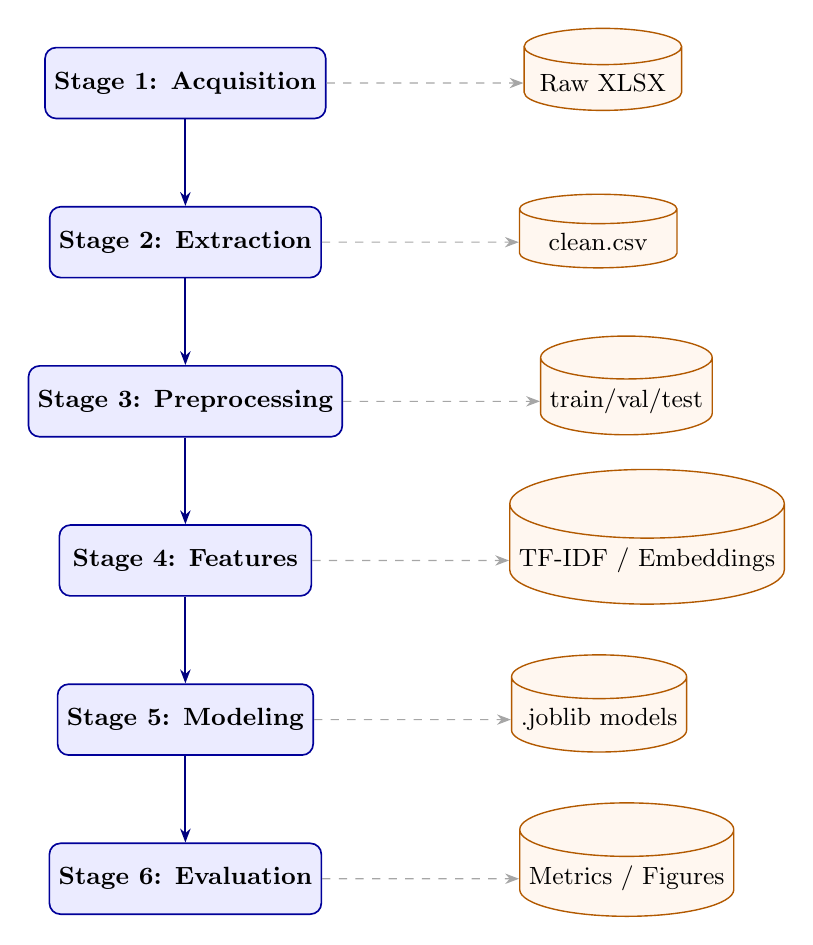
\begin{tikzpicture}[node distance=1.1cm and 0.5cm]

    % Stages
    \node[stage] (s1) {Stage 1: Acquisition};
    \node[stage, below=of s1] (s2) {Stage 2: Extraction};
    \node[stage, below=of s2] (s3) {Stage 3: Preprocessing};
    \node[stage, below=of s3] (s4) {Stage 4: Features};
    \node[stage, below=of s4] (s5) {Stage 5: Modeling};
    \node[stage, below=of s5] (s6) {Stage 6: Evaluation};

    % Data nodes
    \node[data, right=2.5cm of s1] (d1) {Raw XLSX};
    \node[data, right=2.5cm of s2] (d2) {clean.csv};
    \node[data, right=2.5cm of s3] (d3) {train/val/test};
    \node[data, right=2.5cm of s4] (d4) {TF-IDF / Embeddings};
    \node[data, right=2.5cm of s5] (d5) {.joblib models};
    \node[data, right=2.5cm of s6] (d6) {Metrics / Figures};

    % Stage arrows
    \draw[arrow] (s1) -- (s2);
    \draw[arrow] (s2) -- (s3);
    \draw[arrow] (s3) -- (s4);
    \draw[arrow] (s4) -- (s5);
    \draw[arrow] (s5) -- (s6);

    % Data arrows
    \draw[dasharrow] (s1) -- (d1);
    \draw[dasharrow] (s2) -- (d2);
    \draw[dasharrow] (s3) -- (d3);
    \draw[dasharrow] (s4) -- (d4);
    \draw[dasharrow] (s5) -- (d5);
    \draw[dasharrow] (s6) -- (d6);

\end{tikzpicture}
\caption{Six-stage pipeline: each stage produces artefacts consumed by the next.}
\label{fig:pipeline}
\end{figure}

\subsection{Module Architecture}

Figure~\ref{fig:architecture} shows the modular organisation of the \texttt{src/} package, mapping each module to its pipeline stage.

\begin{figure}[H]
\centering
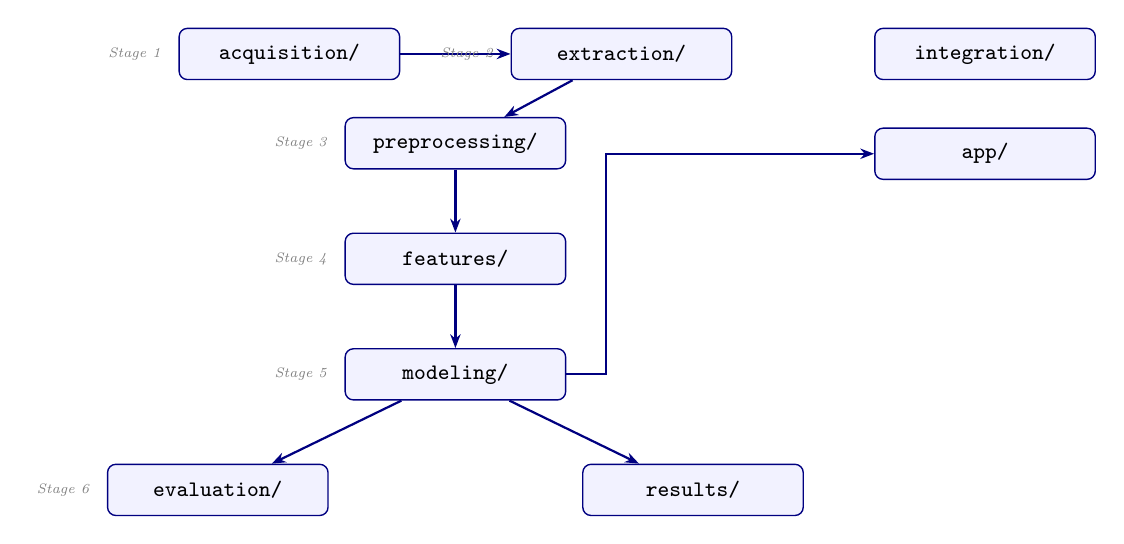
\begin{tikzpicture}[
    node distance=0.6cm and 1.4cm,
    modbox/.style={rectangle, rounded corners=3pt, draw=blue!50!black, fill=blue!5,
                   minimum width=2.8cm, minimum height=0.65cm, font=\footnotesize\ttfamily,
                   line width=0.5pt},
    groupbox/.style={rectangle, rounded corners=5pt, draw=gray!60, dashed,
                     inner sep=8pt, line width=0.5pt}
]

    % Row 1: acquisition + extraction
    \node[modbox] (acq) {acquisition/};
    \node[modbox, right=of acq] (ext) {extraction/};

    % Row 2: preprocessing
    \node[modbox, below=0.8cm of $(acq)!0.5!(ext)$] (pre) {preprocessing/};

    % Row 3: features
    \node[modbox, below=0.8cm of pre] (feat) {features/};

    % Row 4: modeling
    \node[modbox, below=0.8cm of feat] (mod) {modeling/};

    % Row 5: evaluation + results
    \node[modbox, below left=0.8cm and 0.2cm of mod] (eval) {evaluation/};
    \node[modbox, below right=0.8cm and 0.2cm of mod] (res) {results/};

    % Side: integration + app
    \node[modbox, right=1.8cm of ext] (integ) {integration/};
    \node[modbox, below=0.6cm of integ] (app) {app/};

    % Arrows
    \draw[arrow] (acq) -- (ext);
    \draw[arrow] (ext) -- (pre);
    \draw[arrow] (pre) -- (feat);
    \draw[arrow] (feat) -- (mod);
    \draw[arrow] (mod) -- (eval);
    \draw[arrow] (mod) -- (res);
    \draw[arrow] (mod.east) -- ++(0.5,0) |- (app.west);

    % Labels
    \node[font=\tiny\itshape, gray, left=0.1cm of acq] {Stage 1};
    \node[font=\tiny\itshape, gray, left=0.1cm of ext] {Stage 2};
    \node[font=\tiny\itshape, gray, left=0.1cm of pre] {Stage 3};
    \node[font=\tiny\itshape, gray, left=0.1cm of feat] {Stage 4};
    \node[font=\tiny\itshape, gray, left=0.1cm of mod] {Stage 5};
    \node[font=\tiny\itshape, gray, left=0.1cm of eval] {Stage 6};

\end{tikzpicture}
\caption{Module architecture of the \texttt{src/} package, with each module mapped to its pipeline stage. The \texttt{app/} module provides the Flask web interface.}
\label{fig:architecture}
\end{figure}

% ======================================================================
\section{Data Acquisition}
\label{sec:acquisition}
% ======================================================================

\subsection{Corpus: Senti4SD Gold Standard}

The primary dataset is the Senti4SD gold standard~\cite{calefato2018sentiment}, consisting of human-annotated StackOverflow posts labelled for sentiment polarity. The gold-standard workbook (\texttt{Senti4SD\_GoldStandard\_EmotionPolarity.xlsx}) is used rather than Senti4SD's pre-partitioned CSV files because it contains the individual rater columns (\texttt{r1}, \texttt{r2}, \texttt{r3}) required for computing inter-annotator agreement.

\subsection{Corpus Statistics}

\begin{table}[H]
\centering
\caption{Corpus construction summary.}
\label{tab:corpus}
\begin{tabular}{lr}
\toprule
\textbf{Statistic} & \textbf{Value} \\
\midrule
Rows loaded from workbook & 4,423 \\
Duplicate texts dropped & 92 \\
\textbf{Final corpus size} & \textbf{4,331} \\
Fleiss' $\kappa$ & \textbf{0.7586} (4,359 items, 3 raters) \\
Mean document length & 29.97 words \\
Mean sentences per document & 2.33 \\
\bottomrule
\end{tabular}
\end{table}

\begin{table}[H]
\centering
\caption{Class distribution in the Senti4SD corpus.}
\label{tab:classdist}
\begin{tabular}{lrr}
\toprule
\textbf{Class} & \textbf{Count} & \textbf{Share} \\
\midrule
Negative & 1,176 & 27.15\% \\
Neutral  & 1,662 & 38.37\% \\
Positive & 1,493 & 34.47\% \\
\bottomrule
\end{tabular}
\end{table}

The rater columns contain free-text labels with mixed case and typos (\texttt{Postive}, \texttt{Poitive}, \texttt{Netural}); these are repaired programmatically before computing $\kappa$, and items with unparseable rater values are excluded.

\textbf{Implementation:} \texttt{src/acquisition/download.py} fetches the data; \texttt{src/extraction/build\_se.py} performs extraction and quality reporting.

% ======================================================================
\section{Text Extraction and Cleaning}
\label{sec:extraction}
% ======================================================================

A single function, \texttt{clean(text, domain)}, processes all text identically across models. The cleaning pipeline applies the following transformations in strict order:

\begin{enumerate}[leftmargin=*]
    \item \textbf{HTML unescaping} --- handles double-escaped entities (\texttt{\&amp;lt;}).
    \item \textbf{Lowercasing} --- applied \textit{second}, so uppercase placeholders inserted in subsequent steps remain distinguishable from ordinary words.
    \item \textbf{URL replacement} --- \texttt{https?://\textbackslash S+} $\rightarrow$ \texttt{URL}.
    \item \textbf{Mention replacement} --- \texttt{@user} $\rightarrow$ \texttt{USER}.
    \item \textbf{SE domain rules} --- code tags, backtick spans, function calls \texttt{foo(bar)}, and dotted paths \texttt{a.b.c} $\rightarrow$ \texttt{CODE}.
    \item \textbf{Emoticon replacement} --- 17 positive patterns $\rightarrow$ \texttt{EMO\_POS}; 14 negative patterns $\rightarrow$ \texttt{EMO\_NEG}.
    \item \textbf{Negation expansion} --- \texttt{can't} $\rightarrow$ \texttt{can not}, \texttt{won't} $\rightarrow$ \texttt{will not}, etc.
    \item \textbf{Repeated character collapse} --- \texttt{soooo} $\rightarrow$ \texttt{soo}.
    \item \textbf{Whitespace normalisation} --- multiple spaces $\rightarrow$ single space.
\end{enumerate}

\subsection{Critical Order Decisions}

Two ordering choices are load-bearing and merit explicit documentation:

\begin{itemize}[leftmargin=*]
    \item \textbf{Lowercasing before domain rules:} Placeholders (\texttt{URL}, \texttt{CODE}, \texttt{EMO\_POS}) remain uppercase. In the training split, the placeholder \texttt{CODE} occurs in 174 posts and the English word \textit{code} in 303; merging them would produce one meaningless feature spanning 477 posts.
    \item \textbf{URLs before emoticons:} The string \texttt{http://} contains \texttt{:/}, which matches a sad-face emoticon pattern. The reverse order would transform every URL into \texttt{httpEMO\_NEG/...}.
\end{itemize}

\textbf{Stopword removal is disabled permanently.} Negation words (\textit{not}, \textit{no}, \textit{never}) appear in every standard stopword list, and negation flips sentiment.

\textbf{Implementation:} \texttt{src/extraction/clean\_text.py} (211 lines, 36 unit tests). The function \texttt{describe\_rules()} generates the rule table programmatically so the report documentation cannot drift from the code.

% ======================================================================
\section{Preprocessing}
\label{sec:preprocessing}
% ======================================================================

\subsection{Normalisation Modes}

Three normalisation modes are implemented behind a single interface, \texttt{normalize(text, mode)}:

\begin{itemize}[leftmargin=*]
    \item \textbf{\texttt{"none"}} --- tokenise only; words retain their inflections.
    \item \textbf{\texttt{"lemma"}} --- POS-aware lemmatisation via \texttt{WordNetLemmatizer} with tags from \texttt{nltk.pos\_tag}. Without POS tags, \texttt{lemmatize("stopped")} returns \texttt{stopped} (assuming noun), defeating the purpose.
    \item \textbf{\texttt{"stem"}} --- Porter stemming, which is cruder but merges more aggressively (\textit{finally} $\rightarrow$ \textit{final}).
\end{itemize}

All three modes use the \textbf{same tokeniser} (\texttt{TOKEN\_PATTERN}), ensuring the only variable is the word-normalisation step. Placeholders are never touched --- stemming \texttt{CODE} would fold it into the English noun \textit{code}.

\subsection{Normalisation Ablation}

Rather than assuming whether normalisation helps, we \textbf{measured} it. The same model (TF-IDF (1,2) + Logistic Regression at defaults) was trained three times, scored on \textbf{validation}:

\begin{table}[H]
\centering
\caption{Normalisation ablation results on the validation split (650 documents).}
\label{tab:ablation}
\begin{tabular}{lrrrr}
\toprule
\textbf{Mode} & \textbf{Vocabulary} & \textbf{Accuracy} & \textbf{Macro-F1} & \textbf{neut$\rightarrow$neg} \\
\midrule
\textbf{none} & 12,723 & 0.7938 & \textbf{0.7863} & 10.4\% \\
lemma          & 12,186 & 0.7831 & 0.7754 & 11.2\% \\
stem           & 12,371 & 0.7908 & 0.7844 & \textbf{10.0\%} \\
\bottomrule
\end{tabular}
\end{table}

\textbf{Selected: \texttt{none}.} The gap between \texttt{none} and \texttt{stem} is 0.0019 macro-F1, roughly 2 of 650 documents, well inside the noise floor. The defensible justification is that \texttt{none} preserves the inflections the project studies and is simplest. Notably, the two metrics \textbf{disagree}: \texttt{none} wins on macro-F1 while \texttt{stem} has the lowest neutral$\rightarrow$negative rate --- a miniature of the project's central tension between accuracy and interpretability.

\subsection{Data Splitting}

Stratified 70/15/15 splits are created with \texttt{random\_state=42}:

\begin{table}[H]
\centering
\caption{Data split sizes.}
\begin{tabular}{lr}
\toprule
\textbf{Split} & \textbf{Documents} \\
\midrule
Train & 3,031 \\
Validation & 650 \\
Test & 650 \\
\bottomrule
\end{tabular}
\end{table}

Splits are frozen \textbf{before} any model is built. Every vectoriser, embedding, and scaler is fit on \textbf{train only}; fitting on anything else would leak the test set.

\textbf{Implementation:} \texttt{src/preprocessing/normalize.py} (23 tests), \texttt{src/preprocessing/splits.py}.

% ======================================================================
\section{Feature Engineering}
\label{sec:features}
% ======================================================================

\subsection{TF-IDF Representations}

Three TF-IDF configurations are constructed, all sharing \texttt{min\_df=2}, \texttt{max\_df=0.95}, \texttt{sublinear\_tf=True}, and the project's unified \texttt{TOKEN\_PATTERN}. Each vectoriser embeds the \texttt{clean()} and \texttt{normalize()} functions as its preprocessor, so a saved model is a complete pipeline from raw text to prediction.

\begin{table}[H]
\centering
\caption{TF-IDF vocabulary statistics (fitted on training split only).}
\label{tab:tfidf}
\begin{tabular}{lcrrr}
\toprule
\textbf{Config} & \textbf{$n$-grams} & \textbf{Vocabulary} & \textbf{Sparsity} & \textbf{Features/doc} \\
\midrule
\texttt{tfidf11} & (1,1) & 3,449  & 0.9931 & 23.7 \\
\texttt{tfidf12} & (1,2) & 12,723 & 0.9968 & 40.7 \\
\texttt{tfidf13} & (1,3) & 17,902 & 0.9974 & 46.7 \\
\bottomrule
\end{tabular}
\end{table}

\textbf{Most distinctive terms per class} (scored by mean weight inside the class minus mean weight outside):

\begin{table}[H]
\centering
\caption{Top distinctive terms per sentiment class.}
\begin{tabular}{ll}
\toprule
\textbf{Class} & \textbf{Top terms} \\
\midrule
Negative & \texttt{EMO\_NEG}, sad, hate, horrible, afraid, terrible \\
Neutral  & ?, \texttt{URL}, how, what, use, see \\
Positive & !, excellent, thanks, great, \texttt{EMO\_POS}, \textit{thanks\,!} \\
\bottomrule
\end{tabular}
\end{table}

\subsection{The Compound-Phrase Finding}

The proposal motivates $n$-grams with SE-specific phrases: \textit{fatal error}, \textit{kill the process}, \textit{null pointer exception}. A critical finding is that \textbf{none of these occurs even once} in the training corpus. Of 14 tested phrases, the 5 absent ones are exactly the canonical jargon examples. What $n$-grams actually capture is \textbf{negation} (\textit{does not}: 124 posts; \textit{not work}: 34) and \textbf{politeness} (\textit{thank you}: 54 positive, 0 elsewhere).

\subsection{Embeddings}

\begin{table}[H]
\centering
\caption{Embedding statistics.}
\label{tab:embed}
\begin{tabular}{lrrrr}
\toprule
\textbf{Embedding} & \textbf{Vocab.} & \textbf{OOV tokens} & \textbf{Empty docs} & \textbf{Placeholders} \\
\midrule
GloVe (pretrained, 100d) & 400,000 & 2.4\% & 9 & none known \\
Word2Vec (self-trained, 100d) & 3,752 & 3.9\% & 0 & all 5 known \\
\bottomrule
\end{tabular}
\end{table}

\textbf{Nearest-neighbour analysis --- the clearest evidence of domain shift:}

\begin{table}[H]
\centering
\caption{Nearest neighbours reveal domain shift in GloVe embeddings.}
\label{tab:neighbours}
\begin{tabular}{lrll}
\toprule
\textbf{Word} & \textbf{Freq.} & \textbf{GloVe neighbours} & \textbf{W2V neighbours} \\
\midrule
kill      & 3  & killing, \textbf{shoot, poison} & activities, clarify \\
crash     & 9  & \textbf{plane, collision, airplane} & bus, modifying \\
error     & 65 & errors, mistake, fault & \textbf{assertion, failed, throws} \\
fatal     & 0  & deadly, \textbf{poisoning} & \textit{OOV} \\
abort     & 0  & \textbf{aborted, fetuses} & \textit{OOV} \\
\bottomrule
\end{tabular}
\end{table}

GloVe places \textit{kill} beside \textit{shoot} and \textit{poison}, \textit{abort} beside \textit{fetuses}, \textit{crash} beside \textit{airplane}. \textbf{A general-English model reading StackOverflow genuinely sees violence and aviation disasters.} Word2Vec's neighbours are mostly noise due to low word frequencies, but \textit{error} (65$\times$) yields sensible domain neighbours, proving the mechanism works given sufficient data.

\textbf{Implementation:} \texttt{src/features/features\_tfidf.py}, \texttt{src/features/features\_embed.py} (33 tests combined).

% ======================================================================
\section{Model Building}
\label{sec:modeling}
% ======================================================================

\subsection{The Model Grid}

Fifteen models are constructed by crossing five representations with three classifier families:

\begin{table}[H]
\centering
\caption{The 15-model grid.}
\label{tab:modelgrid}
\begin{tabular}{lll}
\toprule
\textbf{Representation} & \textbf{Description} & \textbf{Classifiers} \\
\midrule
\texttt{tfidf11} (1,1) & Unigrams only            & MNB, LR, SVM \\
\texttt{tfidf12} (1,2) & Unigrams + bigrams       & MNB, LR, SVM \\
\texttt{tfidf13} (1,3) & Uni- + bi- + trigrams    & MNB, LR, SVM \\
GloVe (100d)            & Pretrained embeddings    & GNB, LR, SVM \\
Word2Vec (100d)         & Corpus-trained embed.    & GNB, LR, SVM \\
\bottomrule
\end{tabular}
\end{table}

Plus two baselines: majority vote and VADER. Two implementation constraints:

\begin{enumerate}[leftmargin=*]
    \item \textbf{\texttt{LinearSVC} has no \texttt{predict\_proba}}, so it is wrapped in \texttt{CalibratedClassifierCV(cv=5)} --- LIME, SHAP, and the web demo all require probability outputs.
    \item \textbf{\texttt{MultinomialNB} cannot accept embeddings} (which contain negative values), so \texttt{GaussianNB} is used for embedding-based generative models.
\end{enumerate}

\subsection{Hyperparameter Tuning}

All tuning is by \texttt{GridSearchCV} with stratified 5-fold cross-validation, scoring by \texttt{f1\_macro}:

\begin{itemize}[leftmargin=*]
    \item \textbf{MNB:} $\alpha \in \{0.01, 0.1, 0.5, 1.0\}$
    \item \textbf{GNB:} \texttt{var\_smoothing} $\in \{10^{-9}, 10^{-7}, 10^{-5}, 10^{-3}\}$
    \item \textbf{LR:} $C \in \{0.01, 0.1, 1, 10, 100\}$, \texttt{class\_weight} $\in$ \{None, balanced\}
    \item \textbf{SVM:} $C \in \{0.01, 0.1, 1, 10\}$, \texttt{class\_weight} $\in$ \{None, balanced\}
\end{itemize}

Every saved model is a \textbf{complete sklearn pipeline} taking raw strings and exposing both \texttt{predict()} and \texttt{predict\_proba()}, stored as \texttt{models/se/\{features\}\_\{classifier\}.joblib}.

\textbf{Implementation:} \texttt{src/modeling/models\_tfidf.py}, \texttt{src/modeling/models\_embed.py} (19 tests).

% ======================================================================
\section{Evaluation and Results}
\label{sec:results}
% ======================================================================

\subsection{Baselines}

\begin{table}[H]
\centering
\caption{Baseline performance on the test set.}
\begin{tabular}{lrrr}
\toprule
\textbf{Model} & \textbf{Accuracy} & \textbf{Macro-F1} & \textbf{neut$\rightarrow$neg} \\
\midrule
Majority vote & 0.385 & 0.185 & --- \\
VADER         & 0.715 & 0.708 & \textbf{25.2\%} \\
\bottomrule
\end{tabular}
\end{table}

VADER --- a general-purpose lexicon that has never seen a StackOverflow post --- calls \textbf{one in four} genuinely neutral posts negative. This is the problem statement, measured, before any model is built.

\subsection{Test-Set Results}

The test split is read \textbf{once}, after all design decisions are final. Table~\ref{tab:results} shows all 15 models plus baselines:

\begin{table}[H]
\centering
\caption{Full test-set results, sorted by macro-F1.}
\label{tab:results}
\footnotesize
\begin{tabular}{llrrrr}
\toprule
\textbf{Model} & \textbf{Kind} & \textbf{Macro-F1} & \textbf{Accuracy} & \textbf{neut$\rightarrow$neg} & \textbf{neg recall} \\
\midrule
\textbf{tfidf13\_svm} & discrim. & \textbf{0.8275} & 0.8308 & 14.4\% & 76.1\% \\
tfidf13\_lr  & discrim. & 0.8233 & 0.8262 & 14.8\% & 76.7\% \\
tfidf12\_lr  & discrim. & 0.8108 & 0.8138 & 14.0\% & 75.0\% \\
tfidf12\_svm & discrim. & 0.8103 & 0.8154 & 12.8\% & 69.3\% \\
tfidf11\_svm & discrim. & 0.8081 & 0.8123 & 12.0\% & 71.0\% \\
tfidf11\_lr  & discrim. & 0.8070 & 0.8092 & 13.6\% & 75.0\% \\
tfidf12\_mnb & gen.     & 0.7601 & 0.7662 & 12.0\% & 62.5\% \\
tfidf13\_mnb & gen.     & 0.7546 & 0.7600 & 13.2\% & 61.9\% \\
tfidf11\_mnb & gen.     & 0.7331 & 0.7400 & 8.4\%  & 56.2\% \\
w2v\_svm     & discrim. & 0.7059 & 0.7138 & 11.6\% & 55.1\% \\
glove\_lr    & discrim. & 0.7054 & 0.7077 & 17.2\% & 63.1\% \\
w2v\_lr      & discrim. & 0.7020 & 0.7046 & 20.4\% & 64.8\% \\
glove\_svm   & discrim. & 0.6936 & 0.7015 & 12.4\% & 52.8\% \\
w2v\_gnb     & gen.     & 0.5813 & 0.5769 & 49.6\% & 89.2\% \\
glove\_gnb   & gen.     & 0.5668 & 0.5677 & 39.2\% & 79.5\% \\
\midrule
\textit{VADER}    & \textit{baseline} & \textit{0.7079} & \textit{0.7154} & \textit{25.2\%} & --- \\
\textit{Majority} & \textit{baseline} & \textit{0.1852} & \textit{0.3846} & --- & --- \\
\bottomrule
\end{tabular}
\end{table}

\subsection{Key Findings}

\textbf{Research Outcome \#1 --- Which representation handles SE vocabulary best?}

\begin{table}[H]
\centering
\caption{Best and mean macro-F1 by representation family.}
\begin{tabular}{lrr}
\toprule
\textbf{Representation} & \textbf{Best} & \textbf{Mean} \\
\midrule
\textbf{TF-IDF} & \textbf{0.8275} & 0.7928 \\
Word2Vec        & 0.7059 & 0.6631 \\
GloVe           & 0.7054 & 0.6553 \\
\bottomrule
\end{tabular}
\end{table}

TF-IDF wins decisively. The $n$-gram range barely matters (\texttt{tfidf11\_lr} 0.8070 vs \texttt{tfidf13\_lr} 0.8233), consistent with the finding that compound SE phrases are absent from the corpus.

\textbf{Research Outcome \#2 --- Generative vs.\ discriminative.}\quad Discriminative models average \textbf{0.7694} macro-F1 against \textbf{0.6792} for generative models. The gap is consistent across all five representations. GaussianNB suffers most (0.57--0.58) because its independence and normality assumptions fit embeddings poorly.

\textbf{A trap worth naming.}\quad \texttt{tfidf11\_mnb} has the lowest neutral$\rightarrow$negative rate (8.4\%) but finds only 56\% of genuinely negative posts. Its low rate reflects reluctance to predict ``negative'' at all --- a model that never does so would score a perfect 0\%. The two columns must always be read together.

\subsection{Error Analysis}

For \texttt{tfidf13\_svm}, 36 of 250 neutral test posts (14.4\%) were predicted negative:

\begin{table}[H]
\centering
\caption{Error categories for neutral$\rightarrow$negative misclassifications.}
\begin{tabular}{lr}
\toprule
\textbf{Tag} & \textbf{Count} \\
\midrule
Other & 17 \\
Mixed or contrastive tone & 13 \\
Contains SE jargon & 5 \\
Short question & 1 \\
\bottomrule
\end{tabular}
\end{table}

Only 5 of 36 errors involve technical jargon --- \textbf{on this corpus, the model's errors are not primarily caused by technical vocabulary}, consistent with the vocabulary being nearly absent.

\textbf{Implementation:} \texttt{src/evaluation/evaluate.py}, \texttt{tools/run\_final\_evaluation.py}.

% ======================================================================
\section{Explainability Analysis}
\label{sec:explainability}
% ======================================================================

\subsection{LIME Explanations}

LIME generates local explanations by perturbing a single input (randomly deleting words), querying the model on thousands of variants, and fitting a small linear model whose weights indicate each token's contribution. Twenty carefully chosen posts are explained individually (5~correct negatives, 5~correct neutrals, 5~characteristic errors, 5~jargon-heavy), and aggregate weights are computed across 150 gold-neutral test posts.

\textbf{Aggregate result:} The tokens pushing hardest toward ``negative'' on neutral posts are:

\begin{center}
\textit{afraid, me, extremely, i, m, am, !, was, very}
\end{center}

These are \textbf{first-person and affective language}, not technical vocabulary. Zero SE jargon lexicon words occur three or more times in the neutral test posts --- the fourth independent confirmation that the technical vocabulary is not in this corpus.

\subsection{SHAP Explanations}

SHAP provides theoretically grounded Shapley-value attributions. For the linear SVM model, \texttt{shap.LinearExplainer} provides exact values. The same 20 instances are explained for direct comparison with LIME.

\textbf{Top SHAP negative-driving tokens:}
\begin{center}
\textit{hate, painful, line, me, pain, afraid, will not, can not, still}
\end{center}

\subsection{LIME--SHAP Agreement}

The Spearman rank correlation between LIME and SHAP token rankings is $\boldsymbol{\rho = 0.872}$ across 80 shared tokens. Two methods with fundamentally different mathematics --- local linear surrogate vs.\ Shapley allocation --- converge on the same account of model behaviour. This is strong evidence that both describe the model rather than their own sampling noise.

\subsection{Stability Analysis}

Across five random seeds on the 20 fixed posts, the mean Jaccard overlap of the top-5 tokens is \textbf{0.907} (sd~0.164). High but not 1.0 --- individual explanations should be read as indicative, while aggregate tables provide the safer evidence.

\textbf{Implementation:} \texttt{src/evaluation/explain\_lime.py} (266 lines), \texttt{src/evaluation/explain\_shap.py}.

% ======================================================================
\section{Stress Test --- The Central Result}
\label{sec:stress}
% ======================================================================

Four independent analyses established that the Senti4SD corpus cannot answer the research question. A purpose-built 60-sentence stress set was constructed to do so:

\begin{itemize}[leftmargin=*]
    \item \textbf{40 harsh-but-neutral} sentences, e.g., ``\textit{Kill the process before restarting the server.}''
    \item \textbf{20 genuine complaints} (10 with SE jargon, 10 without), e.g., ``\textit{The documentation is worthless and the maintainers ignore every issue.}''
    \item \textbf{10 minimal pairs} using the same jargon word with opposite intent, e.g.,\\
    Neutral: ``\textit{The app crashed after the update.}''\\
    Negative: ``\textit{The app crashed again, this update is useless.}''
\end{itemize}

Sentences cover $\geq$20 SE lexicon words, maximum 5 sentences each, with lengths of 5--30 words.

\begin{table}[H]
\centering
\caption{Stress-test results across models (sorted by accuracy).}
\label{tab:stress}
\footnotesize
\begin{tabular}{lrrrrrr}
\toprule
\textbf{Model} & \textbf{FA\,$\downarrow$} & \textbf{Neg R\,$\uparrow$} & \textbf{Jarg.} & \textbf{Plain} & \textbf{Pairs} & \textbf{Acc.} \\
\midrule
glove\_gnb        & \textbf{2.5\%}  & 70\%  & 90\% & 50\% & \textbf{90\%} & 88.3\% \\
\textbf{tfidf13\_svm} & \textbf{7.5\%} & \textbf{75\%} & 80\% & 70\% & 70\% & \textbf{86.7\%} \\
w2v\_gnb          & 10.0\% & 80\%  & 80\% & 80\% & 70\% & 86.7\% \\
tfidf11\_lr       & 7.5\%  & 65\%  & 70\% & 60\% & 60\% & 83.3\% \\
tfidf12\_lr       & 5.0\%  & 50\%  & 70\% & 30\% & 60\% & 80.0\% \\
tfidf12\_svm      & 5.0\%  & 45\%  & 70\% & 20\% & 60\% & 78.3\% \\
tfidf13\_mnb      & 30.0\% & 70\%  & 90\% & 50\% & 50\% & 68.3\% \\
w2v\_lr           & 45.0\% & 65\%  & 60\% & 70\% & 40\% & 58.3\% \\
glove\_svm        & 55.0\% & 75\%  & 90\% & 60\% & 50\% & 55.0\% \\
glove\_lr         & 62.5\% & 85\%  & 100\%& 70\% & 50\% & 53.3\% \\
\textbf{VADER}    & \textbf{70.0\%} & 75\%  & 90\% & 60\% & 40\% & 45.0\% \\
\bottomrule
\end{tabular}
\end{table}

\subsection{The Headline Result}

\textbf{VADER labels 70\% of harsh-but-neutral SE sentences as negative.} The best test model, \texttt{tfidf13\_svm}, labels only \textbf{7.5\%}, while still catching 75\% of genuine complaints.

\subsection{Outcome \#3 --- Lexical Bias Tracks Pretraining}

\begin{table}[H]
\centering
\caption{Mean false-alarm rate by representation --- bias tracks general English exposure.}
\label{tab:bias}
\begin{tabular}{lr}
\toprule
\textbf{Representation} & \textbf{Mean False Alarm} \\
\midrule
VADER (general lexicon)      & \textbf{70\%} \\
GloVe (general English)      & \textbf{40\%} \\
Word2Vec (this corpus)       & \textbf{28\%} \\
TF-IDF (this corpus)         & \textbf{14\%} \\
\bottomrule
\end{tabular}
\end{table}

\textbf{The ordering tracks exactly how much general English each representation carries.} Pretrained GloVe inherits the lexical bias from general English; representations learned on the StackOverflow corpus largely avoid it. This is the project's direct answer to \textit{``Do models rely on domain-appropriate cues or on general-language bias?''} --- the bias is real, inherited from pretraining, and quantifiable.

\textbf{Implementation:} \texttt{data/stress\_test/se\_stress.csv}, \texttt{src/evaluation/stress\_test.py}.

% ======================================================================
\section{Web Application}
\label{sec:webapp}
% ======================================================================

A Flask-based web interface is provided for interactive exploration of the retained pipeline. The server loads the \texttt{tfidf13\_svm} model at startup and exposes the following endpoints:

\begin{itemize}[leftmargin=*]
    \item \texttt{POST /api/predict} --- accepts raw text, returns the predicted label, class probabilities, and LIME token explanations with per-word highlighting.
    \item \texttt{GET /api/results} --- returns the master results table.
    \item \texttt{GET /api/stress} --- returns stress-test metrics and per-sentence predictions.
    \item \texttt{GET /api/examples} --- provides 8 preloaded example sentences spanning SE jargon, genuine complaints, praise, and neutral questions.
\end{itemize}

The interface renders predictions with colour-coded token contributions (red for negative, green for positive, intensity proportional to weight), providing an immediate visual explanation of the model's reasoning.

\textbf{Implementation:} \texttt{app/server.py} (226 lines), launched via \texttt{python -m app.server}.

% ======================================================================
\section{Limitations}
\label{sec:limitations}
% ======================================================================

\begin{enumerate}[leftmargin=*]
    \item \textbf{The corpus does not contain the phenomenon.} \textit{fatal}, \textit{hang}, and \textit{abort} occur zero times; \textit{kill} three times. Four independent analyses confirmed this. The central claim rests on the stress set, not on Senti4SD.

    \item \textbf{The stress set was written by one person} who already knew what the models were expected to get wrong. The minimal pairs are a partial defence, but blind cross-annotation was not performed.

    \item \textbf{Word2Vec quality is limited by corpus size} (3,031 documents). Its neighbour lists are largely noise, as anticipated in the proposal.

    \item \textbf{LIME and SHAP are approximations.} Measured stability is 0.907 mean Jaccard, not 1.0. Individual explanations are indicative, not exact.

    \item \textbf{Single corpus, single domain.} Whether the failure mode generalises to other technical domains (e.g., DevOps, bioinformatics) is untested.

    \item \textbf{No contextual models.} A fine-tuned transformer (e.g., BERT) might substantially reduce or eliminate the lexical bias measured here.

    \item \textbf{Annotation noise.} Fleiss' $\kappa = 0.759$ indicates good but not perfect agreement. Some ``errors'' are disagreements the annotators also had.
\end{enumerate}

% ======================================================================
\section{Conclusion and Future Work}
\label{sec:conclusion}
% ======================================================================

A tuned TF-IDF (1,3) + calibrated linear SVM reaches \textbf{0.8275 test macro-F1} on the Senti4SD corpus, outperforming the VADER baseline by 0.12 points. Discriminative classifiers beat the generative ones decisively (mean 0.7694 vs.\ 0.6792), and TF-IDF beats both embedding families by a wide margin.

The project's more significant contribution is methodological. The standard SE sentiment corpus does not contain the harsh technical vocabulary that motivates SE sentiment research, so the canonical claim cannot be tested on it --- a fact that four independent analyses surfaced. When tested on purpose-built sentences, the bias is unambiguous: its magnitude tracks exactly how much general English the representation carries, from 70\% false alarms for VADER down to 7.5\% for corpus-trained TF-IDF+SVM.

LIME and SHAP confirm that the best model relies on first-person affective language rather than technical vocabulary, achieving a Spearman agreement of 0.872 between the two methods.

\subsection{Future Work}

\begin{enumerate}[leftmargin=*]
    \item \textbf{Contextual models:} Evaluate a fine-tuned transformer (e.g., CodeBERT, BERTOverflow) to determine whether contextual embeddings eliminate the lexical bias or merely reduce it.
    \item \textbf{Better corpus:} Build a corpus containing error-log vocabulary, drawn from bug trackers and CI/CD logs rather than discussion threads.
    \item \textbf{Cross-annotation:} Extend the stress set with blind annotation by multiple annotators.
    \item \textbf{Cross-domain replication:} Test whether the failure mode generalises to other technical domains such as DevOps, security, or bioinformatics.
\end{enumerate}

% ======================================================================
\section*{Reproducibility}
% ======================================================================

Every number in this report is produced by a runnable script. The complete reproduction sequence:

\begin{lstlisting}[language=bash]
pip install -r requirements.txt
python -m src.acquisition.download
python -m src.extraction.build_se
python -m src.preprocessing.splits --domain se
python -m src.modeling.models_tfidf
python -m tools.run_final_evaluation
python -m src.evaluation.stress_test
python -m src.evaluation.explain_lime
python -m src.evaluation.explain_shap
python -m pytest -q               # 123 tests
\end{lstlisting}

The trained pipeline is saved to \texttt{models/se/tfidf13\_svm.joblib}. The web interface is launched via \texttt{python -m app.server}.

% ── References ──
\begin{thebibliography}{9}

\bibitem{calefato2018sentiment}
Calefato, F., Lanubile, F., Maiorano, F., \& Novielli, N. (2018).
Sentiment Polarity Detection for Software Development.
\textit{Empirical Software Engineering}, 23(3), 1352--1382.

\bibitem{ribeiro2016why}
Ribeiro, M.~T., Singh, S., \& Guestrin, C. (2016).
``Why Should I Trust You?'': Explaining the Predictions of Any Classifier.
\textit{Proceedings of the 22nd ACM SIGKDD}, 1135--1144.

\bibitem{lundberg2017unified}
Lundberg, S.~M. \& Lee, S.-I. (2017).
A Unified Approach to Interpreting Model Predictions.
\textit{Advances in Neural Information Processing Systems}, 30.

\bibitem{pennington2014glove}
Pennington, J., Socher, R., \& Manning, C.~D. (2014).
GloVe: Global Vectors for Word Representation.
\textit{Proceedings of EMNLP}, 1532--1543.

\bibitem{mikolov2013distributed}
Mikolov, T., Sutskever, I., Chen, K., Corrado, G.~S., \& Dean, J. (2013).
Distributed Representations of Words and Phrases and their Compositionality.
\textit{Advances in Neural Information Processing Systems}, 26.

\bibitem{ahmed2017senticr}
Ahmed, T., Bosu, A., Iqbal, A., \& Rahimi, S. (2017).
SentiCR: A Customized Sentiment Analysis Tool for Code Review Interactions.
\textit{Proceedings of ASE}, 106--111.

\bibitem{hutto2014vader}
Hutto, C.~J. \& Gilbert, E. (2014).
VADER: A Parsimonious Rule-Based Model for Sentiment Analysis of Social Media Text.
\textit{Proceedings of ICWSM}, 8(1), 216--225.

\end{thebibliography}

\end{document}
